\subsection{Постановка задачи}
1.5. Реализовать алгоритм QR – разложения матриц в виде программы. На его основе разработать программу, реализующую QR – алгоритм решения полной проблемы собственных значений произвольных матриц, задавая в качестве входных данных матрицу и точность вычислений. С использованием разработанного программного обеспечения найти собственные значения матрицы.

{\bfseries Вариант:} 20
\begin{equation}
      \begin{pmatrix}
        6 & 5 & -6\\
        4 & -6 & 9\\
        -6 & 6 & 1
      \end{pmatrix}
\end{equation}
\pagebreak

\subsection{Результаты работы}

\begin{figure}[h!]
\centering
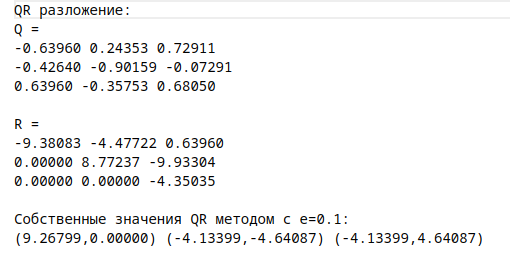
\includegraphics[width=.5\textwidth]{lab1.5}
\caption{Вывод в консоли}
\end{figure}
\pagebreak

\vfill

\subsection{Исходный код}

\lstinputlisting[title=\texttt{5.cpp}]{../stud/svoevolin/exercise_5/5.cpp}
\pagebreak